\section{Sicherheit}
\subsection{Authentifizierung mit OAuth}
\label{oauth}

Die Idee hinter \gls{OAuth} ist bestechend einfach: Eine Applikation möchte auf Dienste im Namen eines Benutzers zugreifen.
Der Benutzer möchte der Applikation sein Passwort jedoch nicht preisgeben, sondern lediglich einige wenige Ressourcen freigeben.
Da sowohl der Benutzer als auch die Applikation dem Anbieter der Ressource vertrauen, kann der Benutzer seinen Anbieter anweisen, der Applikation Zugriff zu gewähren.
Der Anbieter erstellt dazu ein sogenanntes \emph{Access Token}, welches er der Applikation zur Verfügung stellt.

Dieses Prinzip hat auf den ersten Blick nichts mit einem Login zu tun, jedoch kann das Vertrauensverhältnis des Benutzers zum Anbieter und der Applikation zum Anbieter dazu genutzt werden, einen Benutzer einzuloggen, ohne von ihm ein Passwort zu verlangen. 
Die Ressource beinhaltet in diesem Fall die verfügbaren Benutzerinformationen wie Namen, E-Mail Adresse oder ein Profilfoto.

\begin{figure}[H]
	\centering
	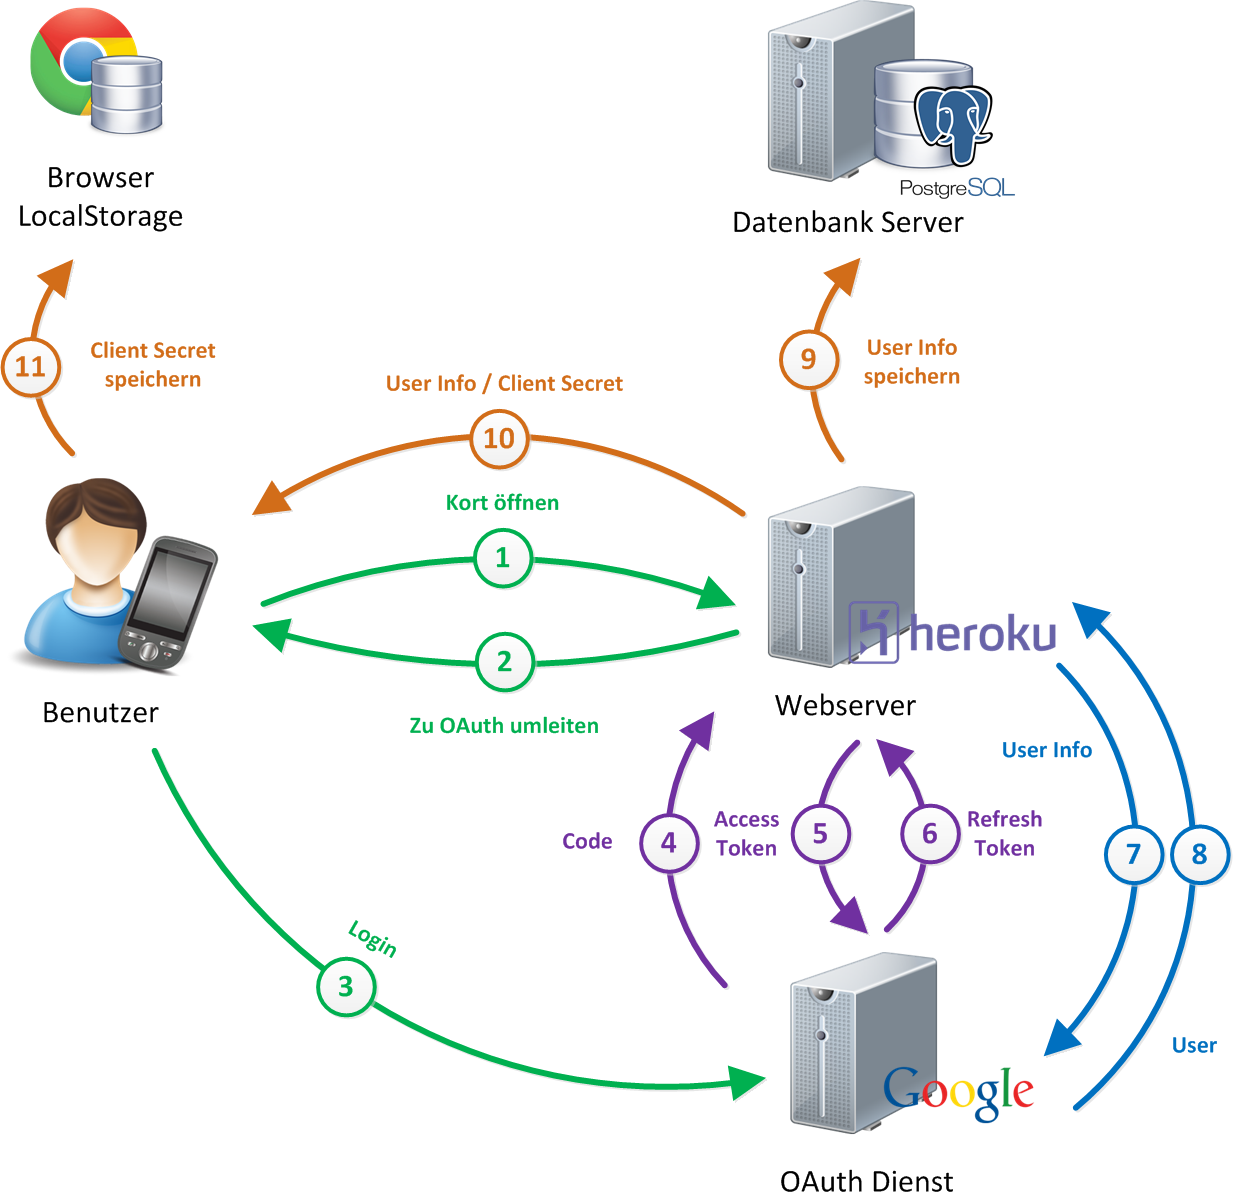
\includegraphics[scale=0.4]{images/implementation/backend/kort-login}
	\caption{Erster Login des Benutzers mit OAuth}
	\label{image-kort-login}
\end{figure}

In unserem Fall ist \kort{} die Applikation und \brand{Google} oder \brand{OpenStreetMap} der Anbieter der \emph{Benutzer}-Ressource.
Um dem Benutzer zu ersparen, sich bei jedem Besuch erneut via \gls{OAuth} anzumelden, wird auf dem Server ein \emph{Secret} generiert.
Dieses wird lokal beim Benutzer gespeichert (siehe Abbildung \ref{image-kort-login}) und ermöglicht es dem Benutzer beim nächsten Login direkt dieses \emph{Secret} zu übermitteln, um Zugriff auf die Applikation zu erhalten (siehe Abbildung \ref{image-kort-relogin}).
Diese Übertragung sollte wenn möglich über SSL/TSL erfolgen.

Wenn der Benutzer erfolgreich eingeloggt wurde, wird dies direkt in der Session des Benutzers gespeichert.
Auf die entsprechenden Werte wird dann bei sicherheitskritischen Abfragen zurückgegriffen.
So ist sichergestellt, dass ein Benutzer lediglich seine eigenen Daten manipulieren kann.

\begin{figure}[H]
	\centering
	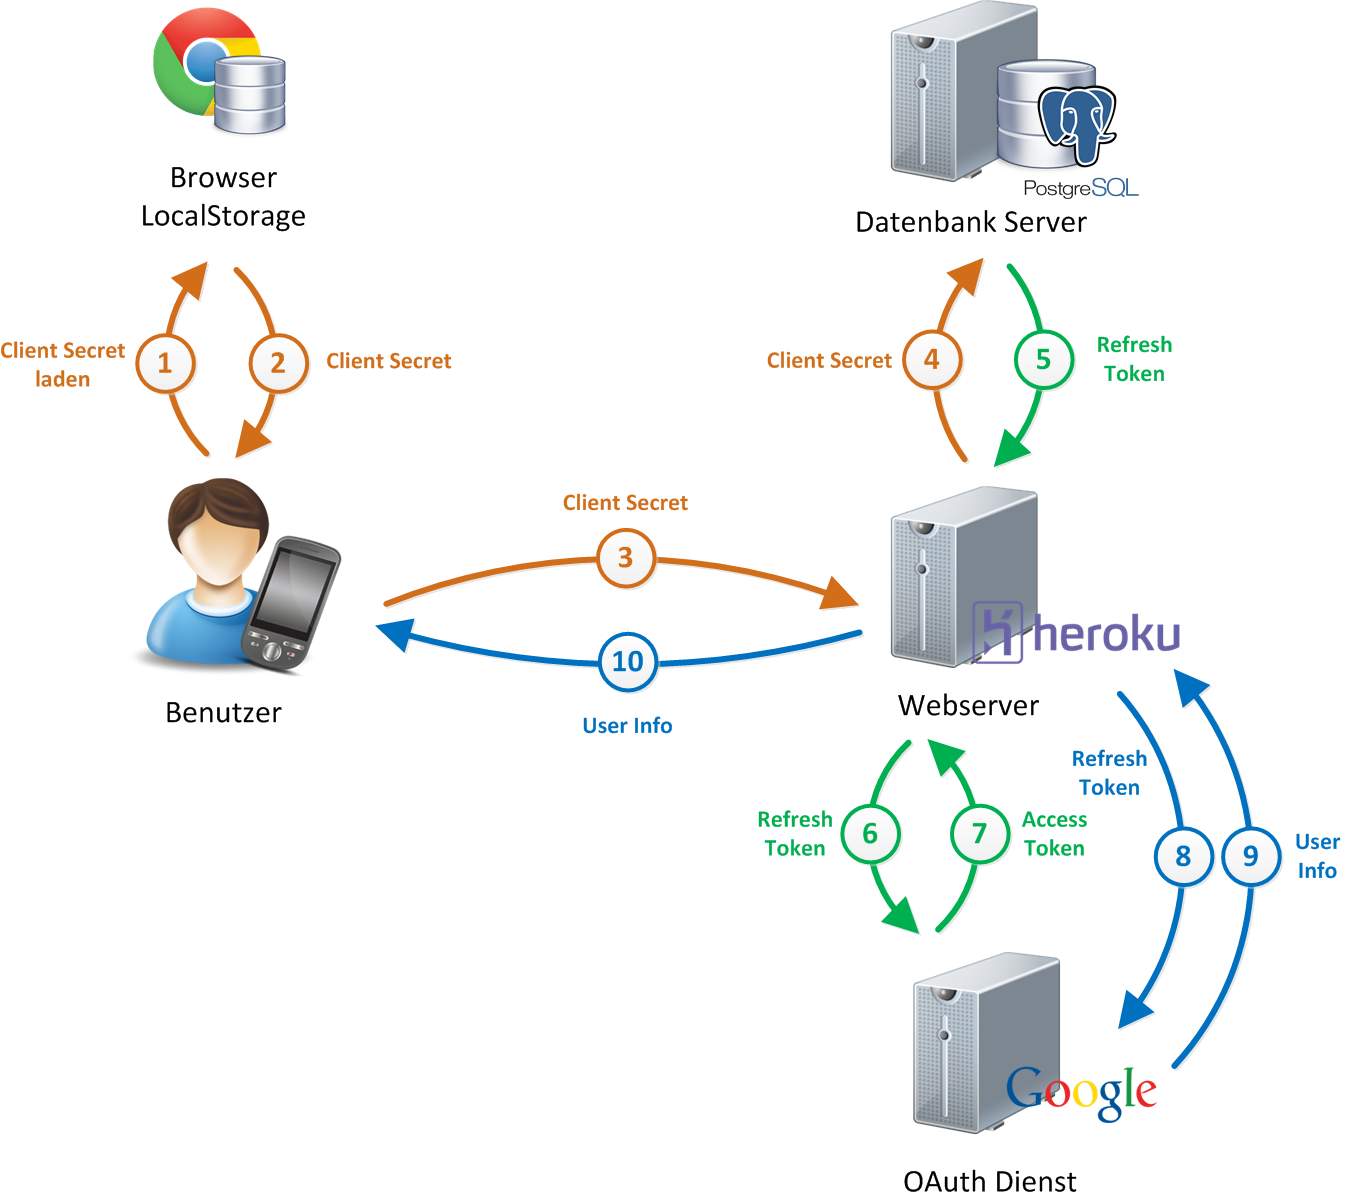
\includegraphics[scale=0.4]{images/implementation/backend/kort-relogin}
	\caption{Wiedererkennen des Benutzers}
	\label{image-kort-relogin}
\end{figure}

\subsubsection{Registrierung der Applikation bei Google}
Um den Google \gls{OAuth} Dienst zu nutzen, muss diese zuerst registriert werden (siehe Abbildung \ref{image-oauth-google-settings}).
Ein Benutzer, der sich einloggen möchte, wird von \kort{} zu Google weitergeleitet.
Von dort wird er nach erfolgter Authentifizierung wieder zurückgeleitet.
Dieses "`Zurückleiten"' wird auch als \emph{Callback} bezeichnet.
Bei der Registrierung der Applikation müssen die gültigen Werte für den Callback definiert werden.

\begin{figure}[H]
	\centering
	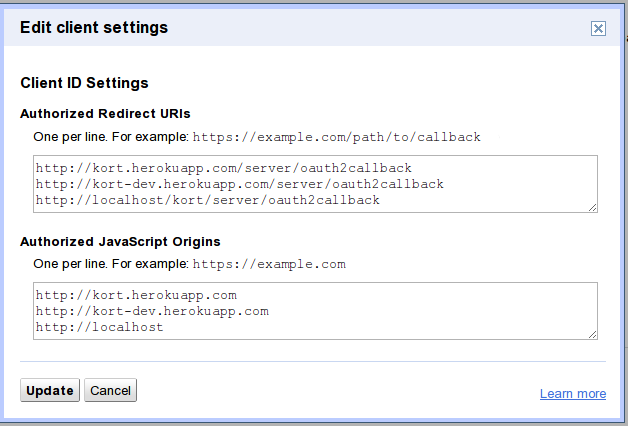
\includegraphics[scale=0.5]{images/implementation/backend/oauth-google-settings}
	\caption{OAuth Einstellungen bei Google}
	\label{image-oauth-google-settings}
\end{figure}

\subsubsection{Registrierung der Applikation bei OpenStreetMap}
Die Registrierung bei \brand{OpenStreetMap} ist sehr ähnlich wie bei Google.
Leider bietet OSM aber keine Möglichkeit, bei einer Registrierung, mehrere URLs anzugeben.
Somit mussten wir für alle unsere Umgebungen (lokal, Entwicklung und Produktion) eine separate Registrierung vornehmen (siehe Abbildung \ref{image-oauth-osm}).

\begin{figure}[H]
	\centering
	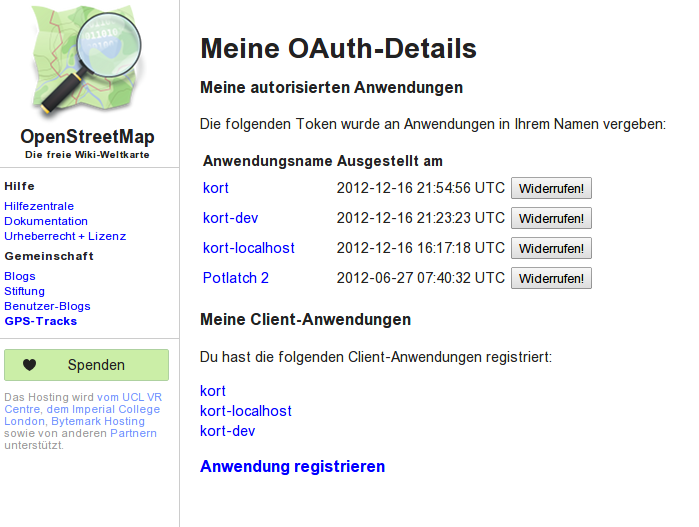
\includegraphics[scale=0.5]{images/implementation/backend/oauth-osm}
	\caption{OAuth Einstellungen bei OpenStreetMap}
	\label{image-oauth-osm}
\end{figure}

\subsection{Übertragungssicherheit}
\label{uebertragunssicherheit}
Die App in der jetzigen Form bietet einige Angriffspunkte.
Die Übertragung über HTTP ermöglicht es einem Angreifer, Nachrichten mitzuhören.
Damit kann er theoretisch die Daten, welche von und zu der Applikation gesendet werden, abfangen und ändern.

Dies ist aus unserer Sicht aber kein grosses Problem, da es sich bei den Applikationsdaten weder um geheime noch besonders schützenswerte Informationen handelt.

Das grösste Risiko ist, dass es unerlaubte Zugriffe auf die Datenbank gibt.
Dazu müsste die Kommunikation zwischen dem Webserver und dem Datenbanksever abgefangen werden.
Der in jedem Request enthaltene \gls{API}-Key für die Datenbank läuft derzeit nicht ab.

Abhilfe würde hier eine Umstellung auf HTTPS (SSL/TLS) schaffen.
Dies erschwert das Mitlesen der Daten erheblich.
Des weiteren könnte die Kommunikation zwischen den Servern mit einem zeitlich generierten Token verbessert werden.
So können auch einfach Replay-Attacken verhindert werden.

Der Fokus dieser Arbeit lag aber nicht darauf, die Server-Server oder Server-Client Kommunikation sicher zu gestalten.
Für den produktiven Einsatz der Applikation müssen in diesem Bereich aber noch Verbesserungen erfolgen.